\hypertarget{lab-02-variables-arrays-and-scripts}{%
\section{Lab 02: Variables, Arrays, and
Scripts}\label{lab-02-variables-arrays-and-scripts}}

\hypertarget{variables}{%
\subsection{Variables}\label{variables}}

\begin{frame}{}
\protect\hypertarget{section}{}
Variables help us represent quantities or expressions in order to make
their use and re-use more convenient.
\end{frame}

\begin{frame}[fragile]{Naming Variables}
\protect\hypertarget{naming-variables}{}
\begin{itemize}[<+->]
\tightlist
\item
  Must start with a letter.
\item
  Followed by letters (a-z, A-Z) or numbers (0-9) or underscores (\_).
\item
  Maximum 65 characters (excluding the .m extension).
\item
  Must not be the same as any MATLAB reserved word.
\item
  Space is not permitted.
\item
  Case sensitive, i.e., \texttt{a\ \textasciitilde{}=\ A}.
\end{itemize}
\end{frame}

\begin{frame}[fragile]{Naming Variables}
\protect\hypertarget{naming-variables-1}{}
\begin{itemize}[<+->]
\tightlist
\item
  Be as descriptive as possible with your variable names.
\item
  Avoid built-in function/variable names (reserved keywords) such as
  \texttt{pi}, \texttt{sin}, \texttt{exp}, etc.
\item
  Check if a name is already in use: \texttt{which\ variableName} or
  \texttt{exist\ variableName}.
\end{itemize}
\end{frame}

\begin{frame}{Naming Conventions}
\protect\hypertarget{naming-conventions}{}
\begin{itemize}[<+->]
\tightlist
\item
  snake\_case: writing compound words or phrases in which the elements
  are separated with one underscore character (\_) and no spaces,
  e.g.~``foo\_bar''.
\item
  camelCase: writing compound words or phrases such that each word or
  abbreviation in the middle of the phrase begins with a capital letter,
  with no intervening spaces or punctuation, e.g.~``fooBar''
\item
  Other conventions: Hungarian notation, positional notation, etc.
\item
  Reference:
  \url{https://en.wikipedia.org/wiki/Naming_convention_(programming)}
\end{itemize}
\end{frame}

\begin{frame}{Default Variable Definitions}
\protect\hypertarget{default-variable-definitions}{}
\begin{table}[!hbtp]
    \begin{tabular}{rl}
        Command & Description \\
        \hline
        \texttt{pi} & variable defining $\pi$ \\
        \texttt{i} or \texttt{1i} & imaginary number $i = \sqrt{-1}$ \\
        \texttt{j} or \texttt{1j} & imaginary number $j = \sqrt{-1}$
    \end{tabular}
\end{table}
\end{frame}

\hypertarget{arrays}{%
\subsection{Arrays}\label{arrays}}

\begin{frame}[fragile]{Array, Vector, and Matrix}
\protect\hypertarget{array-vector-and-matrix}{}
\begin{itemize}[<+->]
\tightlist
\item
  An array is a data form that can hold several values, all of one type.
\item
  A vector is a \(1\)-D array: we can define row vectors, column
  vectors.
\item
  A matrix is a \(2\)-D array.
\item
  Also, we can define \(N\)-D array.
\item
  The general notation for a vector or matrix is a list of values
  enclosed in square brackets \texttt{{[}{]}} separated by commas
  (space) or semi-colons (or the combination).
\end{itemize}
\end{frame}

\begin{frame}[fragile]{Vector: \texttt{{[}{]}}}
\protect\hypertarget{vector}{}
\begin{itemize}[<+->]
\item
  Row vector: \(x = \begin{bmatrix} 1 & 2 & 3 & 4 \end{bmatrix}\)

\begin{verbatim}
x = [1,2,3,4]
x = [1 2 3 4]
\end{verbatim}
\item
  Column vector: \(y = \begin{bmatrix} 1 \\ 2 \\ 3 \\ 4 \end{bmatrix}\)
  or \(y = \begin{bmatrix} 1 & 2 & 3 & 4\end{bmatrix}^{\top}\) or
  \(y = x^{\top}\).

\begin{verbatim}
y = [1;2;3;4]
y = transpose([1 2 3 4])
y = [1 2 3 4]'
y = x'
y = x(:)
\end{verbatim}

  Note: \texttt{\textquotesingle{}} and \texttt{.\textquotesingle{}} are
  the infix notation for \texttt{ctrasnpose}, \texttt{transpose}
  operation.
\end{itemize}
\end{frame}

\begin{frame}[fragile]{Vector: \texttt{linspace} vs.~\texttt{colon}}
\protect\hypertarget{vector-linspace-vs.-colon}{}
\begin{itemize}[<+->]
\item
  \texttt{linspace(from,\ to,\ n)} generates \texttt{n} points between
  \texttt{from} (inclusive) and \texttt{to} (inclusive). For example,

  \texttt{a\ =\ linspace(2,\ 6,\ 5)\ \ \%\ same\ as\ a\ =\ {[}2\ 3\ 4\ 5\ 6{]}}
\item
  \texttt{colon(from,\ step,\ upper\_bound)} generates points between
  \texttt{from} (inclusive) and \texttt{upper\_bound} (may not be
  inclusive) with spacing \texttt{step}. For example,

\begin{verbatim}
a = colon(2, 1, 6)  % same as a = [2 3 4 5 6]
a = colon(2, 2, 6)  % same as a = [2 4 6]
a = colon(2, 1, 7)  % same as a = [2 3 4 5 6 7]
a = colon(2, 2, 7)  % same as a = [2 4 6]
\end{verbatim}
\item
  \texttt{from:step:upper\_bound} is same as
  \texttt{colon(from,\ step,\ upper\_bound)}.
\end{itemize}
\end{frame}

\begin{frame}[fragile]{Vector: \texttt{linspace} vs.~\texttt{colon}}
\protect\hypertarget{vector-linspace-vs.-colon-1}{}
\begin{itemize}[<+->]
\tightlist
\item
  \texttt{linspace(from,\ to,\ n)} is equivalent to
  \texttt{colon(from,\ (to\ -\ from)\ /\ (n\ -\ 1),\ to)}
\item
  \texttt{colon(from,\ step,\ upper\_bound)} is equivalent to
  \texttt{linspace(from,\ floor((upper\_bound\ -\ from)\ /\ step)\ *\ step\ +\ from,\ floor((upper\_bound\ -\ from)\ /\ step))}
\item
  Use \texttt{linspace} when the number of points is given.
\item
  Use \texttt{colon} when the spacing/step size is given.
\end{itemize}
\end{frame}

\begin{frame}[fragile]{Matrix: \texttt{{[}{]}}}
\protect\hypertarget{matrix}{}
Define a \(2 \times 3\) matrix
\(A = \begin{bmatrix} 1 & 2 & 3 \\ 4 & 5 & 6 \end{bmatrix}\)

\begin{verbatim}
A = [1,2,3;4,5,6]
\end{verbatim}

or

\begin{verbatim}
row1 = [1,2,3]
row2 = [4,5,6]
A = [row1;row2]
\end{verbatim}

or

\begin{verbatim}
col1 = [1;4]
col2 = [2;5]
col3 = [3;6]
A = [col1,col2,col3]
\end{verbatim}
\end{frame}

\begin{frame}[fragile]{Matrix: \texttt{zeros}, \texttt{ones},
\texttt{eye}, \texttt{rand}, \texttt{randn}, \texttt{magic}}
\protect\hypertarget{matrix-zeros-ones-eye-rand-randn-magic}{}
\begin{itemize}[<+->]
\item
  \texttt{zeros(m,\ n)}: define a \texttt{m}-by-\texttt{n} matrix with
  zeros.

\begin{verbatim}
zeroRowVec = zeros(5, 1)
zeroColVec = zeros(1, 5)
zeroMatrix = zeros(5, 5)
zeroMatrix = zeros(5)
\end{verbatim}
\item
  \texttt{ones(m,\ n)}: define a \texttt{m}-by-\texttt{n} matrix with
  ones.
\item
  \texttt{eye(m,\ n)}: define a \texttt{m}-by-\texttt{n} matrix with
  diagonals being ones.
\item
  \texttt{rand(m,\ n)}: define a \texttt{m}-by-\texttt{n} matrix with
  uniformly distributed numbers.
\item
  \texttt{randn(m,\ n)}: define a \texttt{m}-by-\texttt{n} matrix with
  normally distributed numbers.
\item
  \texttt{magic(n)}: define a \texttt{n}-by-\texttt{n} magic square with
  row sum, column sum and diagonal sum being equal.
\end{itemize}
\end{frame}

\begin{frame}[fragile]{Dimension: \texttt{size}, \texttt{length},
\texttt{reshape}}
\protect\hypertarget{dimension-size-length-reshape}{}
\begin{itemize}[<+->]
\item
  \texttt{size(array)}: size of \texttt{array}. If \texttt{array} is
  \texttt{n}-dimensional, \texttt{size} will return a vector of length
  \texttt{n}.
\item
  \texttt{size(array,\ 1)}: number of rows of \texttt{array}.
\item
  \texttt{size(array,\ 2)}: number of columns of \texttt{array}.
\item
  \texttt{length(vec)}: length of vector \texttt{vec}, equivalent to
  \texttt{max(size(vec))}.
\item
  \texttt{reshape(array,\ dim1,\ dim2,\ dim3,\ ...)}.

\begin{verbatim}
rowVec = 1:8
matrix = reshape(rowVec, 2, 4)
% same as matrix = [1,3,5,7;2,4,6,8]
\end{verbatim}
\item
  \texttt{reshape(array,\ prod(size(array)),\ 1)} is same as
  \texttt{array(:)}.
\end{itemize}
\end{frame}

\begin{frame}[fragile]{\(N\)-D array: \texttt{reshape}}
\protect\hypertarget{n-d-array-reshape}{}
Define 3-D array:

\begin{verbatim}
rowVec = 1:8
array = reshape(rowVec, 2, 2, 2);
length(size(array))  % check the dimension
\end{verbatim}
\end{frame}

\begin{frame}[fragile]{1-D Array: Slicing}
\protect\hypertarget{d-array-slicing}{}
\begin{itemize}[<+->]
\item
  Define a row vector \texttt{rowVec}:

\begin{verbatim}
rowVec = [2,4,6,8,10]
rowVec = linspace(2,10,5)
rowVec = colon(2,2,10)    % or rowVec = 2:2:10
\end{verbatim}
\item
  \texttt{array(i)}: the \texttt{i}-th entry of \texttt{array}, where
  \texttt{i} is called the index:

  \begin{table}[!hbtp]
    \centering
    \begin{tabular}{cccccc}
      \toprule
      \verb|i|         & 1 & 2 & 3 & 4 & 5 \\
      \midrule
      \verb|rowVec(i)| & 2 & 4 & 6 & 8 & 10 \\
      \bottomrule
    \end{tabular}
  \end{table}
\end{itemize}
\end{frame}

\begin{frame}[fragile]{1-D Array: Slicing}
\protect\hypertarget{d-array-slicing-1}{}
\begin{table}[!hbtp]
  \centering
  \begin{tabular}{cccccc}
    \toprule
    \verb|i|         & 1 & 2 & 3 & 4 & 5 \\
    \midrule
    \verb|rowVec(i)| & 2 & 4 & 6 & 8 & 10 \\
    \bottomrule
  \end{tabular}
\end{table}

\begin{itemize}[<+->]
\item
  Extract one entry from a vector: For example, to extract \texttt{6}
  from \texttt{rowVec} and assign it to \texttt{x}:

  \texttt{x\ =\ rowVec(3)}
\item
  Extract multiple entries from a vector: For example, to extract
  \texttt{2}, \texttt{6}, \texttt{8} from \texttt{rowVec} and assign it
  to \texttt{x}:

  \texttt{x\ =\ rowVec({[}1,3,4{]})}
\item
  Extract multiple continguous entries from a vector: For example, to
  extract \texttt{4}, \texttt{6}, \texttt{8} from \texttt{rowVec} and
  assign it to \texttt{x}:

\begin{verbatim}
x = rowVec([2,3,4])
x = rowVec(2:4)
\end{verbatim}
\end{itemize}
\end{frame}

\begin{frame}[fragile]{2-D array: Slicing}
\protect\hypertarget{d-array-slicing-2}{}
\begin{itemize}[<+->]
\item
  Define a matrix \texttt{mat}

\begin{verbatim}
mat = reshape(1:8, 2, 4)
\end{verbatim}
\item
  \texttt{array(i,\ j)}: the entry of \texttt{array} at row \texttt{i}
  and column \texttt{j}, where \texttt{i} is colled row index,
  \texttt{j} is called column index:

  \begin{table}[!hbtp]
    \centering
    \begin{tabular}{c|cccc}
      \toprule
      \diagbox{\texttt{i}}{\texttt{mat(i, j)}}{\texttt{j}} & 1 & 2 & 3 & 4 \\
      \hline
      1 & 1 & 3 & 5 & 7 \\
      2 & 2 & 4 & 6 & 8 \\
      \bottomrule
    \end{tabular}
  \end{table}
\end{itemize}
\end{frame}

\begin{frame}[fragile]{2-D array: Slicing}
\protect\hypertarget{d-array-slicing-3}{}
\begin{table}[!hbtp]
  \centering
  \begin{tabular}{c|cccc}
    \toprule
    \diagbox{\texttt{i}}{\texttt{mat(i, j)}}{\texttt{j}} & 1 & 2 & 3 & 4 \\
    \hline
    1 & 1 & 3 & 5 & 7 \\
    2 & 2 & 4 & 6 & 8 \\
    \bottomrule
  \end{tabular}
\end{table}

Extract multiple rows and multiple columns from \texttt{mat}: For
example, to extract entries at row \texttt{1}, row \texttt{2}, and
column \texttt{2}, column \texttt{4}:

\begin{verbatim}
A = mat([1,2], [2,4])
A = mat(1:2, [2,4])
A = mat(1:end, [2,4])
A = mat(:, [2,4])
\end{verbatim}
\end{frame}

\begin{frame}[fragile]{Generate a \(3\)-D Array using Slicing}
\protect\hypertarget{generate-a-3-d-array-using-slicing}{}
\begin{verbatim}
slice1 = [1,2;3,4]
slice2 = [5,6;7,8]
C(:,:,1) = slice1
C(:,:,2) = slice2
\end{verbatim}
\end{frame}

\begin{frame}[fragile]{Concatenate Arrays}
\protect\hypertarget{concatenate-arrays}{}
\begin{verbatim}
row1 = [1,2,3]
row2 = [4,5,6]
rowVec = [row1,row2]  % rowVec = [1,2,3,4,5,6]
matrix = [row1;row2]  % matrix = [1,2,3;4,5,6]
matrix1 = [matrix1;matrix2]
% same as matrix1 = [1,2,3;4,5,6;1,2,3;4,5,6]
matrix2 = [matrix1,matrix2]
% same as matrix2 = [1,2,3,1,2,3;4,5,6,4,5,6]
\end{verbatim}
\end{frame}

\begin{frame}[fragile]{1-D Array: Append/Delete Element}
\protect\hypertarget{d-array-appenddelete-element}{}
\begin{verbatim}
% 1-D array
rowVec = 1:5
rowVec(end + 1) = 6  % append 6 to rowVec
rowVec = [rowVec,7]  % append 7 to rowVec
rowVec(5) = []       % delete 5 from rowVec
rowVec(2:4) = []     % delete 2, 3, 4 from rowVec
\end{verbatim}
\end{frame}

\begin{frame}[fragile]{2-D Array: Append/Delete Element}
\protect\hypertarget{d-array-appenddelete-element-1}{}
\begin{verbatim}
% 2-D array
matrix = magic(5)
matrix(:, end + 1) = 1:5   % append a column vector
matrix = [matrix,[6:10]']  % append a column vector
matrix(end + 1, :) = 1:7   % append a row vector
matrix = [matrix;8:14]     % append a row vector
matrix(:,6) = []           % delete column 2
matrix(:,3:5) = []         % delete column 3, 4, 5
matrix(2:4,:) = []         % delete row 2, 3, 4
\end{verbatim}
\end{frame}

\begin{frame}[fragile]{Char Array vs.~String Array}
\protect\hypertarget{char-array-vs.-string-array}{}
\begin{verbatim}
str = "abc"
arrayOfChars1 = 'abc'
arrayOfChars2 = ['a','b','c']
arrayOfChars1 == arrayOfChars2 % return logical 1 (true)
arrayOfChars1 == str           % return logical 1 (true)
class(str)                     % string
class(arrayOfChars1)           % char
[arrayOfChars1,arrayOfChars2]  % return 'abcabc'
[arrayOfChars1;arrayOfChars2]  % return ['abc';'abc']
[str,str]                      % return ["abc","abc"]
[str;str]                      % return ["abc";"abc"]
\end{verbatim}
\end{frame}

\begin{frame}[fragile]{Cell Array: array of elements of different types}
\protect\hypertarget{cell-array-array-of-elements-of-different-types}{}
\begin{itemize}[<+->]
\item
  \texttt{cell(n)}: create 1-D cell array of length \texttt{n}
\item
  \texttt{cell(m,n)}: create 2-D cell array of size \texttt{m} by
  \texttt{n}
\item
  Create a cell array of types \texttt{char}, \texttt{string},
  \texttt{double}:

\begin{verbatim}
cellArray = {[1,2,3], "abc", 'def'}
cellArray{1}          % return [1,2,3]
cellArray{2}          % return "abc"
cellArray{3}          % return 'def'
cellArray{4} = 'ghi'
cellArray{4}          % return 'ghi'
\end{verbatim}
\end{itemize}
\end{frame}

\begin{frame}[fragile]{Array Operations: 1-D Array}
\protect\hypertarget{array-operations-1-d-array}{}
\begin{itemize}[<+->]
\tightlist
\item
  \texttt{sum(vec)}/\texttt{prod(vec)}: sum/product of all elements of
  \texttt{vec}.
\item
  \texttt{max(vec)}/\texttt{min(vec)}: maximum/minimum of \texttt{vec}.
\item
  \texttt{rowVec\ =\ rowVec1\ .*\ rowVec2}: elementwise multiplication,
  where \texttt{rowVec(i)\ =\ rowVec1(i)\ *\ rowVec2(i)}.
\item
  \texttt{rowVec\ .*\ colVec}: Kronecker product. If \texttt{rowVec} has
  length \texttt{m} and \texttt{colVec} has length \texttt{n}, then the
  resulting matrix is \texttt{m}-by-\texttt{n}.
\item
  \texttt{dot(vec1,\ vec2)}: dot product of \texttt{vec1} and
  \texttt{vec2}, \texttt{vec1} and \texttt{vec2} must be of the same
  length.
\item
  \texttt{sum(rowVec1\ .*\ rowVec2)}: \texttt{dot(rowVec1,\ rowVec2)}.
\item
  \texttt{rowVec1\ *\ rowVec2\textquotesingle{}}:
  \texttt{dot(rowVec1,\ rowVec2)}.
\item
  \texttt{indices\ =\ find(vec\ \textgreater{}\ n)}: find indices of
  elements greater than \texttt{n} in \texttt{vec}. Note:
  \texttt{\textgreater{}} can also be \texttt{\textless{}}, \texttt{==}.
\end{itemize}
\end{frame}

\begin{frame}[fragile]{Array Operations: 2-D Array}
\protect\hypertarget{array-operations-2-d-array}{}
\begin{itemize}[<+->]
\tightlist
\item
  \texttt{mat\ =\ mat1\ .*\ mat2}: elementwise multiplication, where
  \texttt{mat(i,\ j)\ =\ mat1(i,\ j)\ *\ mat2(i,\ j)}.
\item
  \texttt{mat\ =\ mat1\ *\ mat2}: matrix multiplication, where
  \texttt{mat1} is \texttt{m}-by-\texttt{p}, \texttt{mat2} is
  \texttt{p}-by-\texttt{n}, and \texttt{mat} is
  \texttt{m}-by-\texttt{n}.
\item
  \texttt{sum/prod(mat,\ \textquotesingle{}all\textquotesingle{})}:
  sum/product of all elements of \texttt{mat}.
\item
  \texttt{sum/prod(mat,\ 1)}: column sums/products.
\item
  \texttt{sum/prod(mat,\ 2)}: row sums/products.
\item
  \texttt{max/min(mat,\ {[}{]},\ \textquotesingle{}all\textquotesingle{})}:
  maximum/minimum of \texttt{mat}.
\item
  \texttt{max/min(mat,\ {[}{]},\ 1)}: column maximums/minimums.
\item
  \texttt{max/min(mat,\ {[}{]},\ 2)}: row maximums/minimums.
\item
  \texttt{{[}row,\ col{]}\ =\ find(mat\ \textgreater{}\ n)}: find
  indices of elements greater than \texttt{n} in \texttt{mat},
  \texttt{row}/\texttt{col} stores row/column indices.
\end{itemize}
\end{frame}

\begin{frame}[fragile]{Array Operations: 2-D Array}
\protect\hypertarget{array-operations-2-d-array-1}{}
\begin{itemize}[<+->]
\tightlist
\item
  \texttt{{[}V,\ D{]}\ =\ eig(mat)}: \texttt{V(:,\ i)} and
  \texttt{D(i,\ i)} are the \texttt{i}-th eigenvector and eigenvalue of
  \texttt{mat}.
\item
  \texttt{d\ =\ diag(mat,\ k)}: extract \texttt{k}-th diagonal elements
  that is above (\texttt{k\ \textgreater{}\ 0}) / below
  (\texttt{k\ \textless{}\ 0}) the main diagonal.
\item
  \texttt{mat\ =\ diag(d,\ k)}: construct a matrix with \texttt{k}-th
  diagonal elements being \texttt{d}.
\item
  \texttt{mat\ =\ diag(diag(mat,\ k))}: set elements to zero except the
  \texttt{k}-th diagonal elements.
\item
  \texttt{fliplr(mat)}: flip \texttt{mat} in left/right direction.
\item
  \texttt{flipud(mat)}: flip \texttt{mat} in up/down direction.
\item
  \texttt{rot90(mat,\ k)}: rotate \texttt{mat} \texttt{k\ *\ 90}
  degrees.
\end{itemize}
\end{frame}

\begin{frame}[fragile]{Application: Image Processing}
\protect\hypertarget{application-image-processing}{}
\begin{itemize}[<+->]
\item
  A grayscale image is a 2-D array of pixels, each pixel has a integer
  value that represent depth of color.
\item
  A colored image is a 3-D array of pixels with RGB channels, each
  channel is a 2-D array.
\item
  \texttt{img\ =\ imread(filename)}: read image from graphics file
  \texttt{filename} and assign it \texttt{img}.
\item
  \texttt{imshow(img)}: display image \texttt{img} in handle graphics
  figure.
\item
  \texttt{imwrite(img,\ filename)}: write image \texttt{img} to graphics
  file named \texttt{filename}.

\begin{verbatim}
uw = imread('UW.png');
uwFlipud = flipud(uw);
imshow(uwFlipud);
imwrite(uwFlipud, 'UW_flipud.png');
\end{verbatim}
\end{itemize}
\end{frame}

\begin{frame}{Summary}
\protect\hypertarget{summary}{}
\begin{table}[!hbtp]
  \begin{tabular}{rl}
    Command                          & Description \\
    \hline
    \texttt{transpose} or \texttt{'} & Non-conjugate transpose of a vector \\
    \texttt{linspace}                & Linearly spaced vector \\
    \texttt{logspace}                & Logarithmically spaced vector \\
    \texttt{colon} or \texttt{:}     & Colon \\
    \texttt{zeros}                   & Zeros array \\
    \texttt{ones}                    & Ones array \\
    \texttt{eye}                     & Identity matrix \\
    \texttt{rand}                    & Uniformly distributed pseudorandom numbers \\
    \texttt{randn}                   & Normally distributed pseudorandom numbers \\
    \texttt{magic}                   & Magic square \\
    \texttt{size}                    & Size of array \\
    \texttt{length}                  & Length of vector \\
    \texttt{reshape}                 & Reshape array \\
  \end{tabular}
\end{table}
\end{frame}

\begin{frame}{Summary}
\protect\hypertarget{summary-1}{}
\begin{table}[!hbtp]
  \begin{tabular}{rl}
    Command                          & Description \\
    \hline
    \texttt{diag}                    & Diagonal matrices and diagonals of a matrix \\
    \texttt{cell}                    & Create cell array \\
    \texttt{sum}/\texttt{prod}       & Sum/Product of elements \\
    \texttt{min}/\texttt{max}        & Minimum/Maximum of elements \\
    \texttt{dot}                     & Vector dot product \\
    \texttt{find}                    & Find indices of nonzero elements \\
    \texttt{eig}                     & Find eigenvalues and eigenvectors \\
    \texttt{diag}                    & Diagonal matrices and diagonals of a matrix \\
    \texttt{fliplr}/\texttt{flipud}  & Flip an array \\
    \texttt{rot90}                   & Rotate an array 90 degrees \\
    \texttt{imread}/\texttt{imwrite} & Read/Write image from graphics file \\
    \texttt{imshow}                  & display image in Handle Graphics figure \\
    \texttt{uint8}                   & Convert to unsigned 8-bit integer \\
  \end{tabular}
\end{table}
\end{frame}

\begin{frame}{Additional Commands}
\protect\hypertarget{additional-commands}{}
\begin{table}[!hbtp]
  \begin{tabular}{rl}
    Command            & Description \\
    \hline
    \texttt{iskeyword} & Check if input is a keyword \\
    \texttt{who}       & List current variables \\
    \texttt{whos}      & List current variables, long form \\
    \texttt{which}     & Locate functions and files \\
    \texttt{clear}     & Clear variables and functions from memory \\
    \texttt{clc}       & Clear command window \\
    \texttt{clf}       & Clear current figure \\
    \texttt{close}     & Close figure \\
    \texttt{exist}     & Check existence of variable/script/function/folder/class \\
    \texttt{disp}      & Display array \\
  \end{tabular}
\end{table}
\end{frame}

\hypertarget{script-files}{%
\subsection{Script Files}\label{script-files}}

\begin{frame}{}
\protect\hypertarget{section-1}{}
A script file is simply a file that contains a chain of commands that
you edit in a separate window, then execute with a single mouse click or
command. This is where we can define variables, perform calculations and
leave comments to remind us what the file calculates.
\end{frame}

\begin{frame}{File Naming Conventions}
\protect\hypertarget{file-naming-conventions}{}
\begin{itemize}[<+->]
\tightlist
\item
  Start with a letter, followed by letters or numbers or underscore,
  maximum 63 characters (excluding the .m extension), and must not be
  the same as any MATLAB reserved word.
\item
  None of the conventions matter to MATLAB itself: they only matter to
  the people writing the code, and the people maintaining the code
  (usually a much harder task), and to the people paying for the code
  (you'd be amazed how much gets written into contract specifications.)
\item
  Reference:
  \url{https://www.mathworks.com/matlabcentral/answers/30223-what-are-the-rules-for-naming-script-files}
\end{itemize}
\end{frame}

\begin{frame}[fragile]{Put Comments to Your Script File}
\protect\hypertarget{put-comments-to-your-script-file}{}
\begin{verbatim}
% MATH 3341, Semester Year
% Lab 02: Variables, Arrays, and Scripts
% Author: first_name last_name
% Date: mm/dd/yyyy
\end{verbatim}
\end{frame}

\begin{frame}{Useful MATLAB Shortcuts}
\protect\hypertarget{useful-matlab-shortcuts}{}
\begin{itemize}[<+->]
\tightlist
\item
  Windows shortcuts

  \begin{itemize}[<+->]
  \tightlist
  \item
    Press \fbox{\texttt{Ctrl}} + \fbox{\texttt{A}} to select all
  \item
    Press \fbox{\texttt{Ctrl}} + \fbox{\texttt{I}} to adjust indentation
  \item
    Press \fbox{\texttt{Ctrl}} + \fbox{\texttt{R}} to comment
  \item
    Press \fbox{\texttt{Ctrl}} + \fbox{\texttt{T}} to uncomment
  \end{itemize}
\item
  macOS shortcuts

  \begin{itemize}[<+->]
  \tightlist
  \item
    Press \fbox{\texttt{command}} + \fbox{\texttt{A}} to select all
  \item
    Press \fbox{\texttt{command}} + \fbox{\texttt{I}} to adjust
    indentation
  \item
    Press \fbox{\texttt{command}} + \fbox{\texttt{/}} to comment
  \item
    Press \fbox{\texttt{command}} + \fbox{\texttt{T}} to uncomment
  \end{itemize}
\end{itemize}
\end{frame}

\hypertarget{primer}{%
\subsection{\texorpdfstring{\LaTeX~Primer}{~Primer}}\label{primer}}

\begin{frame}[fragile]{\texttt{table} Environment}
\protect\hypertarget{table-environment}{}
\begin{verbatim}
\begin{table}[!hbtp]
  \caption{This is a table}
  \begin{tabular}{rcl}
  \toprule
  Column 1 & Column 2 & Column 3 \\
  \midrule
  1        & 1        & 1        \\
  12       & 12       & 12       \\
  123      & 123      & 123      \\
  \bottomrule
  \end{tabular}
\end{table}
\end{verbatim}
\end{frame}

\begin{frame}{\texttt{table} Environment}
\protect\hypertarget{table-environment-1}{}
\begin{table}[!hbtp]
  \caption{This is a table}
  \begin{tabular}{rcl}
  \toprule
  Column 1 & Column 2 & Column 3 \\
  \midrule
  1        & 1        & 1        \\
  12       & 12       & 12       \\
  123      & 123      & 123      \\
  \bottomrule
  \end{tabular}
\end{table}
\end{frame}

\begin{frame}[fragile]{\texttt{figure} Environment}
\protect\hypertarget{figure-environment}{}
\begin{verbatim}
\begin{figure}[!hbtp]
  \centering
  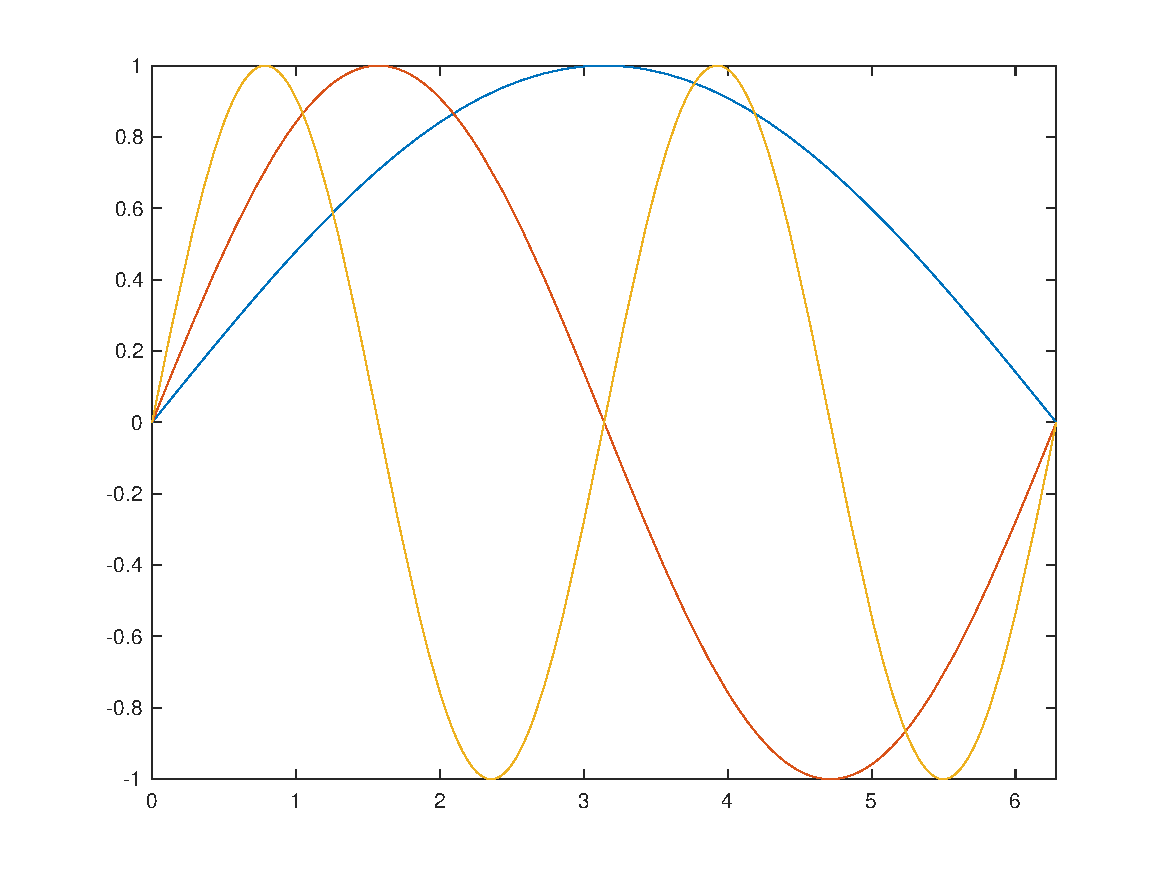
\includegraphics[height=0.3\textheight]{figure.pdf}
  \caption{Plot of $\sin{x}$}
  \label{fig:sin}
\end{figure}
\end{verbatim}

generates

\begin{figure}[!hbtp]
  \centering
  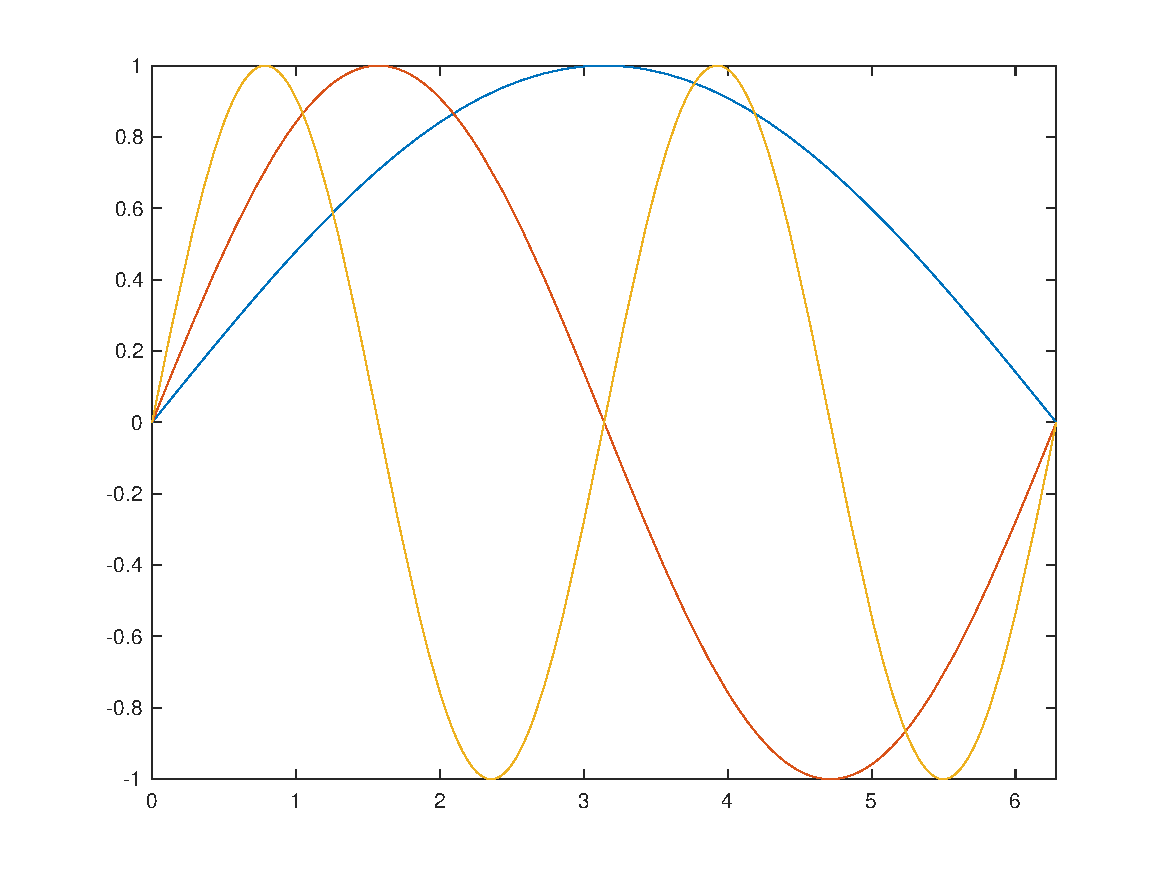
\includegraphics[height=0.3\textheight]{figure.pdf}
  \caption{Plot of $\sin{x}$}
  \label{fig:sin}
\end{figure}
\end{frame}

\begin{frame}[fragile]{\texttt{\textbackslash{}left} and
\texttt{\textbackslash{}right} vs.~\texttt{\textbackslash{}big},
\texttt{\textbackslash{}Big}, \texttt{\textbackslash{}Bigg}}
\protect\hypertarget{left-and-right-vs.-big-big-bigg}{}
\begin{verbatim}
\begin{align*}
\|x\|_2 & = \big(\sum_{i = 1}^{n} x_i^2 \big)^{1/2},
\|x\|_2 = \Big(\sum_{i = 1}^{n} x_i^2 \Big)^{1/2}, \\
\|x\|_2 & = \Bigg(\sum_{i = 1}^{n} x_i^2 \Bigg)^{1/2},
\|x\|_2 = \left(\sum_{i = 1}^{n} x_i^2 \right)^{1/2}.
\end{align*}
\end{verbatim}

generates \begin{align*}
\|x\|_2 & = \big(\sum_{i = 1}^{n} x_i^2 \big)^{1/2},
\|x\|_2 = \Big(\sum_{i = 1}^{n} x_i^2 \Big)^{1/2}, \\
\|x\|_2 & = \Bigg(\sum_{i = 1}^{n} x_i^2 \Bigg)^{1/2},
\|x\|_2 = \left(\sum_{i = 1}^{n} x_i^2 \right)^{1/2}.
\end{align*}
\end{frame}

\begin{frame}[fragile]{Links}
\protect\hypertarget{links}{}
\begin{verbatim}
\href{https://www.google.com}{Google}
\end{verbatim}

\href{https://www.google.com}{Google}

Or simply

\begin{verbatim}
\url{https://www.google.com}
\end{verbatim}

\url{https://www.google.com}
\end{frame}

\begin{frame}[fragile]{\texttt{case} Environment}
\protect\hypertarget{case-environment}{}
\begin{verbatim}
$$
f(x) =
\begin{cases}
5 x + 4   & \text{if~} x \leq 1, \\
3 x^2 + 6 & \text{if~} x > 1
\end{cases}
$$
\end{verbatim}

generates \[
f(x) =
\begin{cases}
5 x + 4   & \text{if~} x \leq 1, \\
3 x^2 + 6 & \text{if~} x > 1
\end{cases}
\]
\end{frame}

\begin{frame}[fragile]{Cross-Reference}
\protect\hypertarget{cross-reference}{}
\begin{verbatim}
\begin{equation}
\label{eq:ls}
A \mathbf{x} = \mathbf{b}.
\end{equation}

The expression \eqref{eq:ls} is a linear system.
\end{verbatim}

generates

\begin{equation}
\label{eq:ls}
A \mathbf{x} = \mathbf{b}.
\end{equation}

The expression \eqref{eq:ls} is a linear system.
\end{frame}

\begin{frame}[fragile]{Cross-Reference}
\protect\hypertarget{cross-reference-1}{}
\begin{verbatim}
\begin{table}[!hbtp]
\caption{$y = 2x$}
\label{tab:xy}
  \begin{tabular}{cc}
  \toprule
  $x$ & $y$ \\
  \midrule
  $6$ & $12$ \\
  $7$ & $14$ \\
  $8$ & $16$ \\
  \bottomrule
  \end{tabular}
\end{table}
Table \ref{tab:xy} gives the result of $y = 2x$.
\end{verbatim}
\end{frame}

\begin{frame}{Cross-Reference}
\protect\hypertarget{cross-reference-2}{}
\begin{table}[!hbtp]
\caption{$y = 2x$}
\label{tab:xy}
  \begin{tabular}{cc}
  \toprule
  $x$ & $y$ \\
  \midrule
  $6$ & $12$ \\
  $7$ & $14$ \\
  $8$ & $16$ \\
  \bottomrule
  \end{tabular}
\end{table}

Table \ref{tab:xy} gives the result of \(y = 2x\).
\end{frame}
